\documentclass[a4]{article}
\usepackage{amssymb,amsmath}
\usepackage[mathscr]{eucal}
\usepackage{graphicx}

\newcommand{\id}{{\mathbb I}}
\newcommand{\tr}{{\rm tr}\,}
\parskip=1em
\begin{document}

\section{Cloning}

\subsection{Setup for perfect probabilistic cloning \boldmath $m\to n$}

Assume $|\psi_1\rangle$, $|\psi_2\rangle$, as well as their prior probabilities $\eta_1$, $\eta_2$ are known. Perfect cloning is given by a unitary $U$ such that
$$
U|\psi_i\rangle^m|0\rangle=\sqrt p_i |\psi_i\rangle^n|s\rangle+\sqrt q_i |\phi\rangle|f\rangle,\quad i=1,2,
$$
where $|s\rangle$ and $|f\rangle$ stand for success and failure, $\langle s| f\rangle=0$; $|0\rangle$, $|s\rangle$ and $|f\rangle$ are some ancillary states and $|\phi\rangle$ is the (garbage) state produced upon failure to clone.

Unitarity implies
$$
p_i+q_i=1,\quad i=1,2,
$$
and
$$
s^m=\sqrt{p_1p_2}s^n+\sqrt{q_1 q_2}, \quad n>m,
$$
where $s=\langle\psi_1|\psi_2\rangle$ is the overlap. We can choose $s>0$ without loss of generality.

\subsection{Unitarity curve}\label{uni cur}

We write $\sqrt{p_i}=\cos\theta_i$, $0\le\theta_i\le\pi/2$, thus $\sqrt q_i=\sin\theta_i$. The unitarity constraint becomes
$$
s^m={\cos(\theta_1+\theta2)+\cos(\theta_1-\theta_2)\over2} s^n-{\cos(\theta_1+\theta2)-\cos(\theta_1-\theta_2)\over2}.
$$
Define $x=\cos(\theta_1+\theta_2)$ and $y=\cos(\theta_1-\theta_2)$, then the previous equation is
$$
s^m=-{1-s^n\over 2}x+{1+s^n\over2}y;\quad -1\le x\le1,\; 0\le y\le 1.
$$
This is the equation of a straight line. In parametric form it may be written as
$$
x={1-(1+s^n)t\over s^{n-m}},\qquad y={1-(1-s^n)t \over s^{n-m}},
$$
where
$$
{1-s^{n-m}\over 1-s^n}\le t\le {1\over1-s^n};\quad  {1-s^{n-m}\over 1+s^n}\le t\le {1+s^{n-m}\over1+s^n},
$$
which can be combined to give
$$
{1-s^{n-m}\over 1-s^n}\le t\le \min\left\{{1\over1-s^n},{1+s^{n-m}\over1+s^n}\right\}.
$$
Then
%
\begin{eqnarray*}
\sqrt p_1&=&\cos\left\{{1\over2}\arccos{1-(1+s^n)t\over s^{n-m}}+{1\over2}\arccos{1-(1-s^n)t\over s^{n-m}}\right\},\\[1em]
\sqrt p_2&=&\cos\left\{{1\over2}\arccos{1-(1+s^n)t\over s^{n-m}}-{1\over2}\arccos{1-(1-s^n)t\over s^{n-m}}\right\}.
\end{eqnarray*}
%
(For $\sqrt q_1$ and $\sqrt q_2$ we just replace $\sin$ for $\cos$.) We note that for $t>1$ we have~$\sqrt p_1<0$, as the argument of $\cos$ on the right hand side becomes larger than~$\pi/2$. Hence, the allowed range of $t$ is~\footnote{The value $t=1$ is most easily found by inspection. For $t=1$, the argument of $\cos$ in the expression of $\sqrt p_1$ reads 
$$
{1\over2}\arccos(-s^m)+{1\over2}\arccos(s^m)={\pi\over2}
$$
for any value of $s^m>0$.
}
$$
{1-s^{n-m}\over 1-s^n}\le t\le  1.
$$
Finally, the region is manifestly symmetric under $p_1\leftrightarrow p_2$. Its shape, of course, is {\em independent} of the priors $\eta_1$ and $\eta_2$. Some examples are ($m=1$, $n=2$):
$$
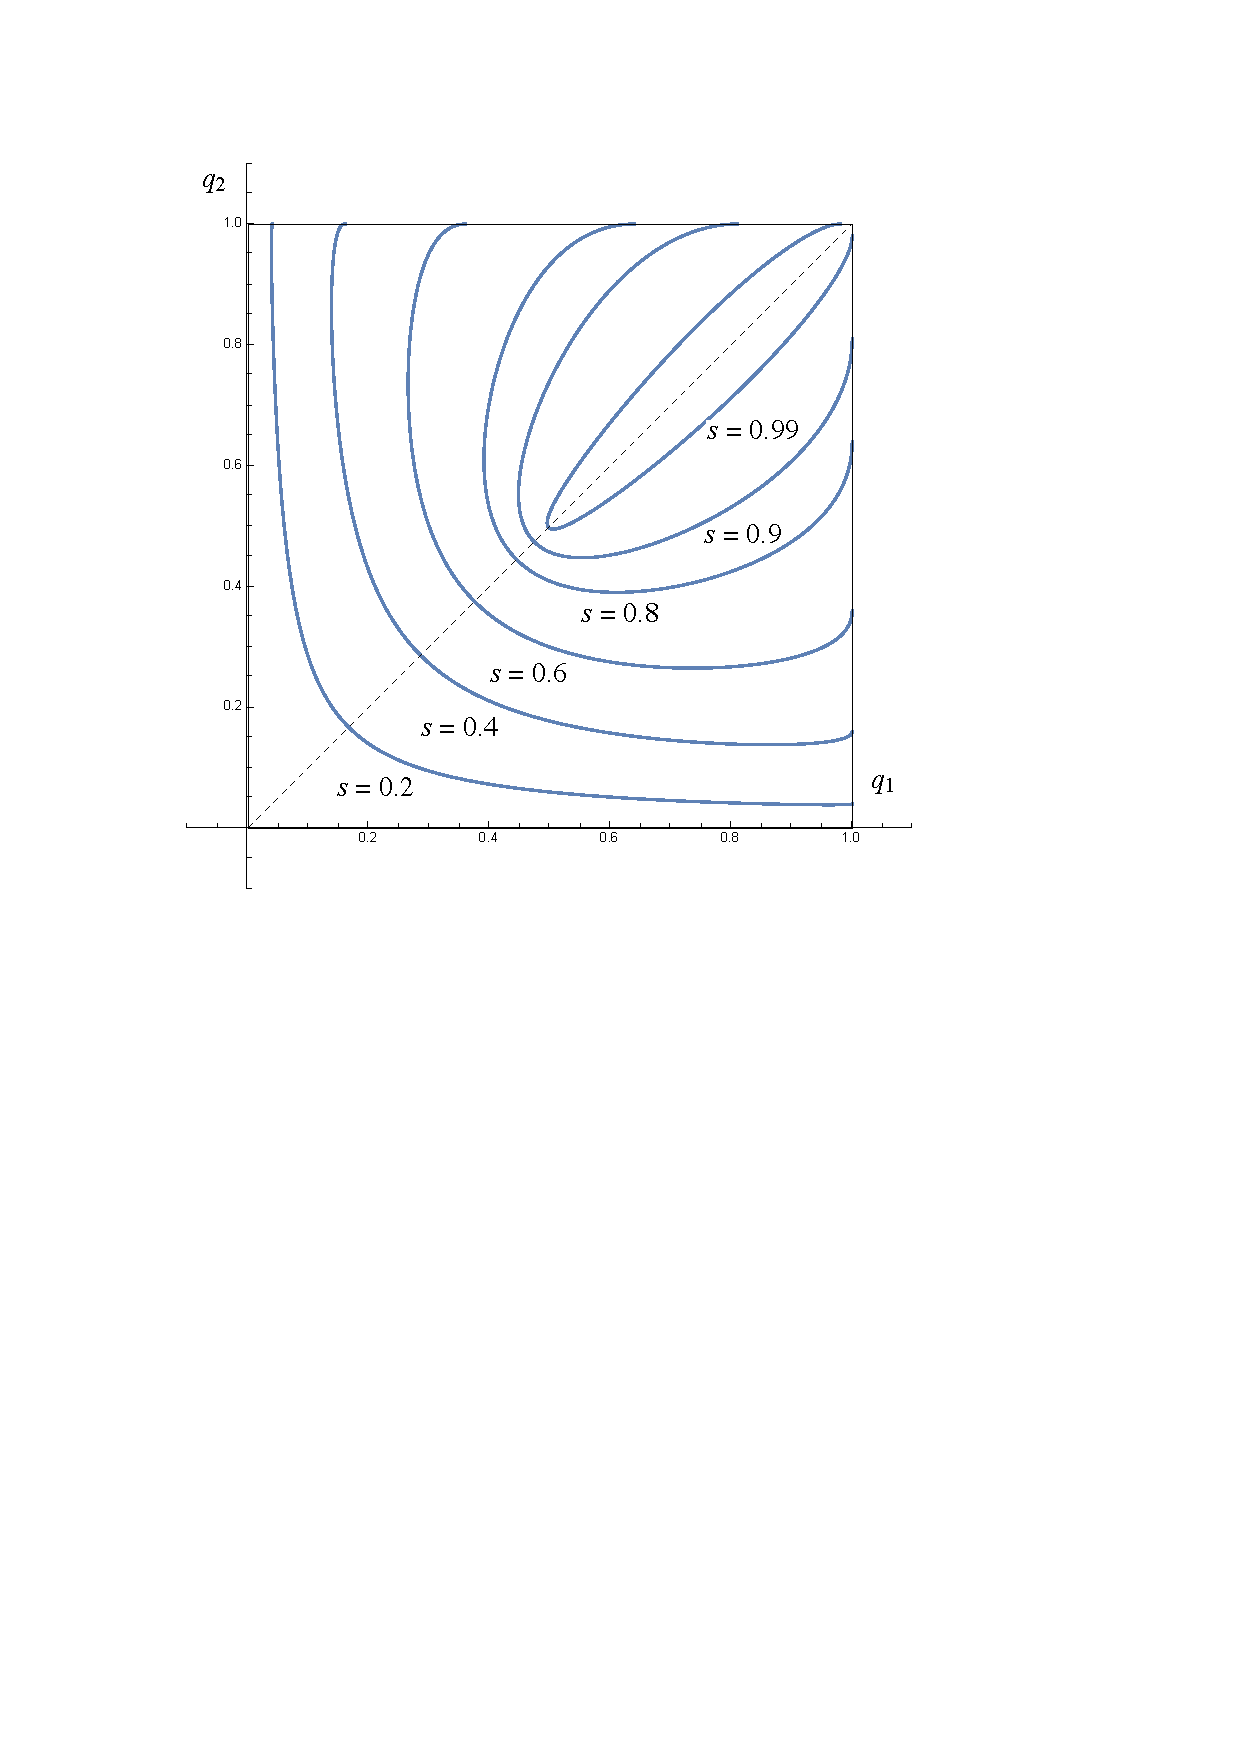
\includegraphics[width=22em]{Andi4_F1.pdf}
$$
Note that we can easily get rid of the trigonometric functions and write
%
\begin{eqnarray*}
p_1&=&{1+xy-\sqrt{1-x^2}\sqrt{1-y^2}\over2},\\[.2em]
p_2&=&{1+xy+\sqrt{1-x^2}\sqrt{1-y^2}\over2}.
\end{eqnarray*}
%
or, equivalently
%
\begin{eqnarray*}
q_1&=&{1-xy+\sqrt{1-x^2}\sqrt{1-y^2}\over2},\\[.2em]
q_2&=&{1-xy-\sqrt{1-x^2}\sqrt{1-y^2}\over2}.
\end{eqnarray*}
%

\subsection{Minimization}

Our objective function is the average failure probability
$$
Q=\eta_1 q_1+\eta_2 q_2 .
$$
We view this as the equation of a straight line in the plane defined by $q_1$ and $q_2$ with normal vector $\vec n=(\eta_1,\eta_2)$. Since, $\eta_1$ and $\eta_2$ are probabilities, $\vec n$ belongs in the first quadrant. The minimum $Q$ is  that for which the corresponding straight line is tangent to the unitarity curve. Then
$$
\eta_1 q'_1+\eta_2 q'_2=0.
$$
Using that $1=\eta_1+\eta_2$ we have
$$
\eta_1={q'_2\over q'_2-q'_1},\quad \eta_2={q'_1\over q'_1-q'_2}.
$$
These equations define $\eta_1$ and $\eta_2$ in parametric form. 
Since the problem is symmetric under $1\leftrightarrow2$, it is sufficient to consider the range $0\le\eta_1\le 1/2$.
Then,
$$
0=\eta_1\;\Rightarrow\; q'_2=0\;\Rightarrow\; {d\over dt}\sqrt{q_2}=0
$$
gives the maximum value of $t$. We obtain
$$
0={d\over dt}\sqrt{q_2}={\sqrt p_2\over2s^{n-m}}\left({1+s^n\over\sqrt{1-x^2}}-{1-s^n\over\sqrt{1-y^2}}\right).
$$
Thus, the term in parenthesis must vanish. This gives
$$
t_{\rm max}={1-s^{2(n-m)}\over1-s^{2n}}<1.
$$
We also have the inequality,
$$
t_{\rm min}\equiv {1-s^{n-m}\over1-s^n}\le{1-s^{n-m}\over1-s^n}{1+s^{n-m}\over1+s^n}={1-s^{2(n-m)}\over1-s^{2n}}
=t_{\rm max} .
$$
Substituting back into $q_2$ we get that the minimum $q_2=Q$ is
$$
Q_{\rm min}=q_{2,{\rm min}}={s^{2m}-s^{2n}\over 1-s^{2n}}.
$$
The maximum value of $Q$ is at $t_{\rm min}$. Substituting in the expression of $Q$ we obtain
$$
Q_{\rm max}={s^m-s^n\over1-s^n}.
$$

For intermediate values of $t$,  $t_{\rm min}<t<t_{\rm max}$, we can plot the parametric curve given by
$$
(\eta_1,Q)=\left({q'_2\over q'_2-q'_1},{q'_2\over q'_2-q'_1}q_1+{q'_1\over q'_1-q'_2}q_2\right).
$$
One can check that
%
\begin{eqnarray*}
q'_1&=&{\sqrt{q_1(1-q_1)}\over s^{n-m}}\left({1+s^n\over\sqrt{1-x^2}}+{1-s^n\over\sqrt{1-y^2}}\right),\\[.25em]
q'_2&=&{\sqrt{q_2(1-q_2)}\over s^{n-m}}\left({1+s^n\over\sqrt{1-x^2}}-{1-s^n\over\sqrt{1-y^2}}\right).
\end{eqnarray*}
The next figure is a plot of $Q$ vs. $\eta_1$ for the same values of $s$ used in the previous figure.
$$
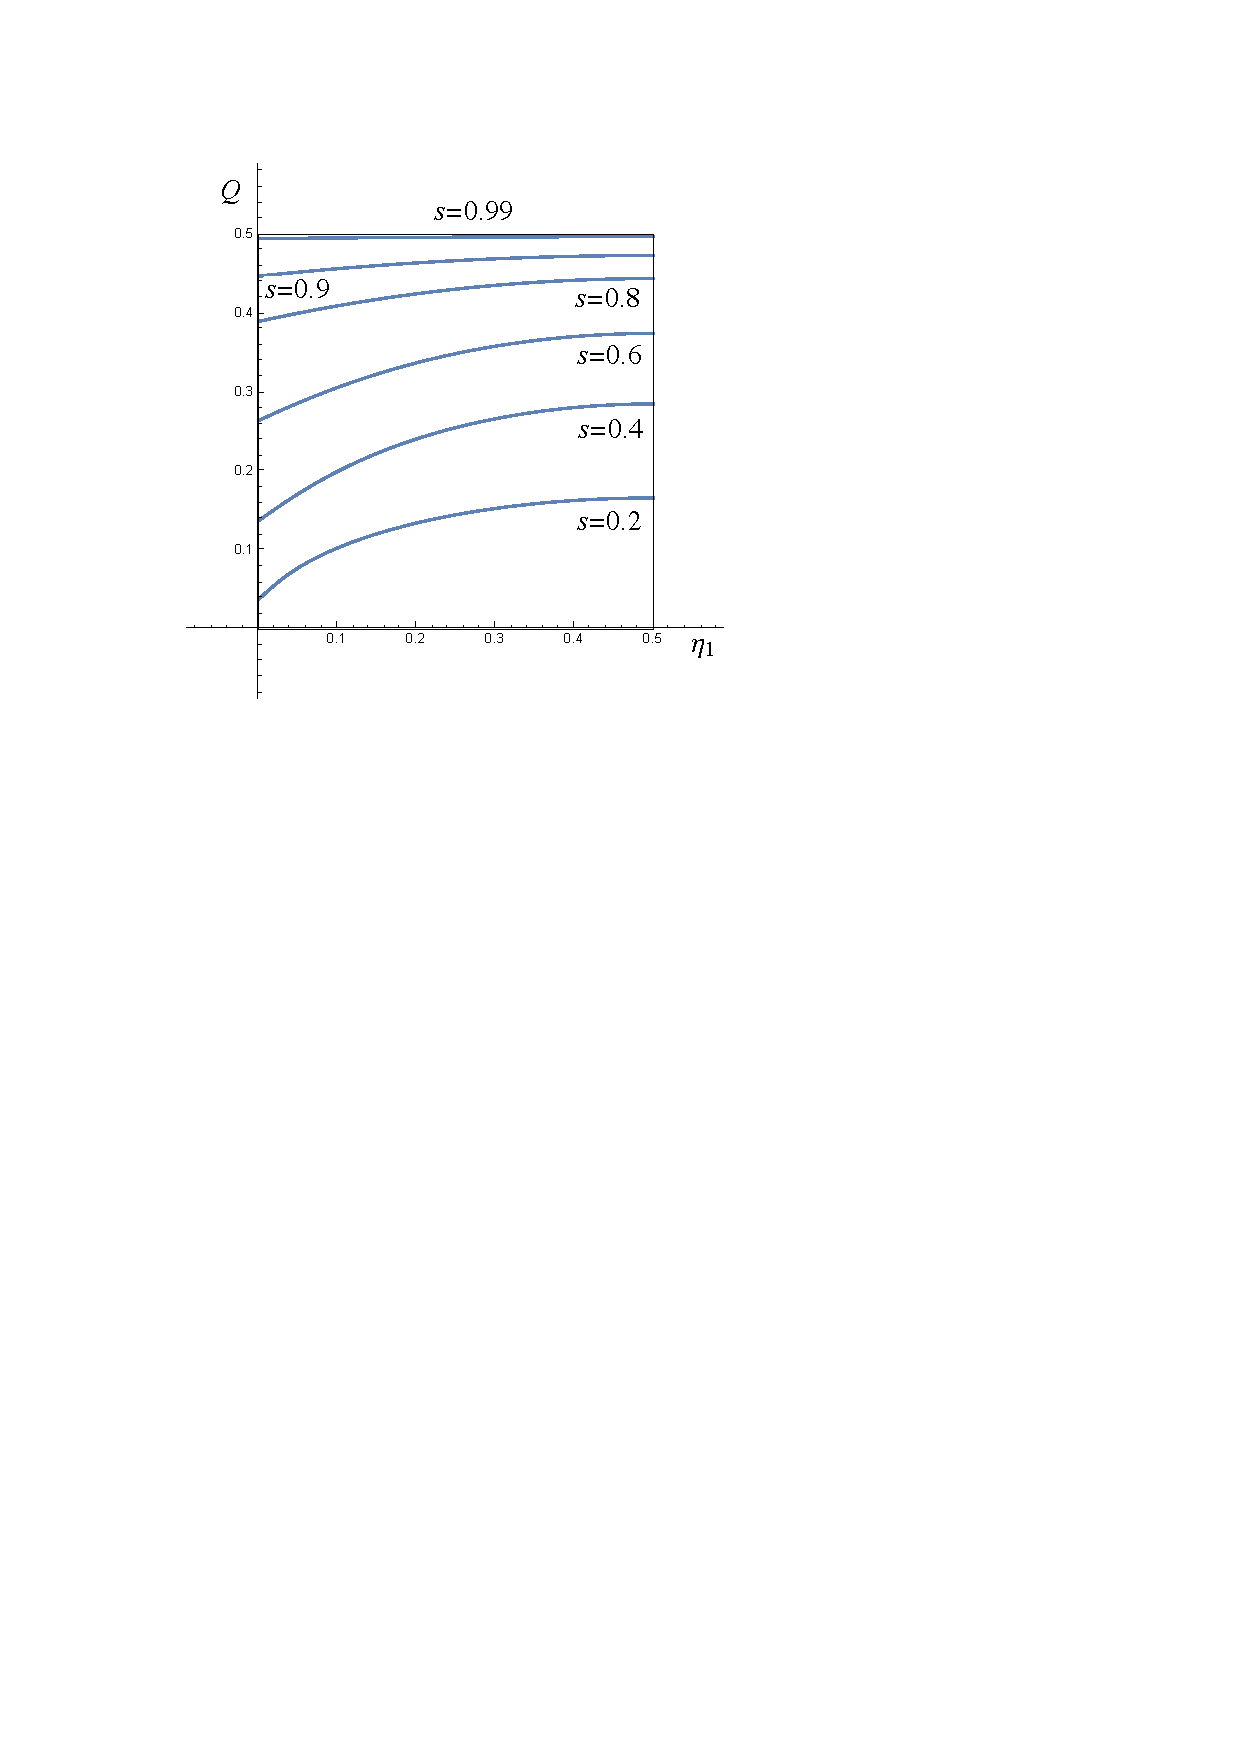
\includegraphics[width=22em]{Andi4_F2.pdf}
$$

\subsection{Information leakage and suboptimality of unambiguous discrimination}

We observed that a discrimination protocol consisting of cloning followed by optimal discrimination is suboptimal except if $\eta_1=0,1/2,1$. Vadim would like to link this to the leaking of information at the cloning stage. Some ideas concerning this follow.

Let us start with the most simple scenario shown in the figure.
$$
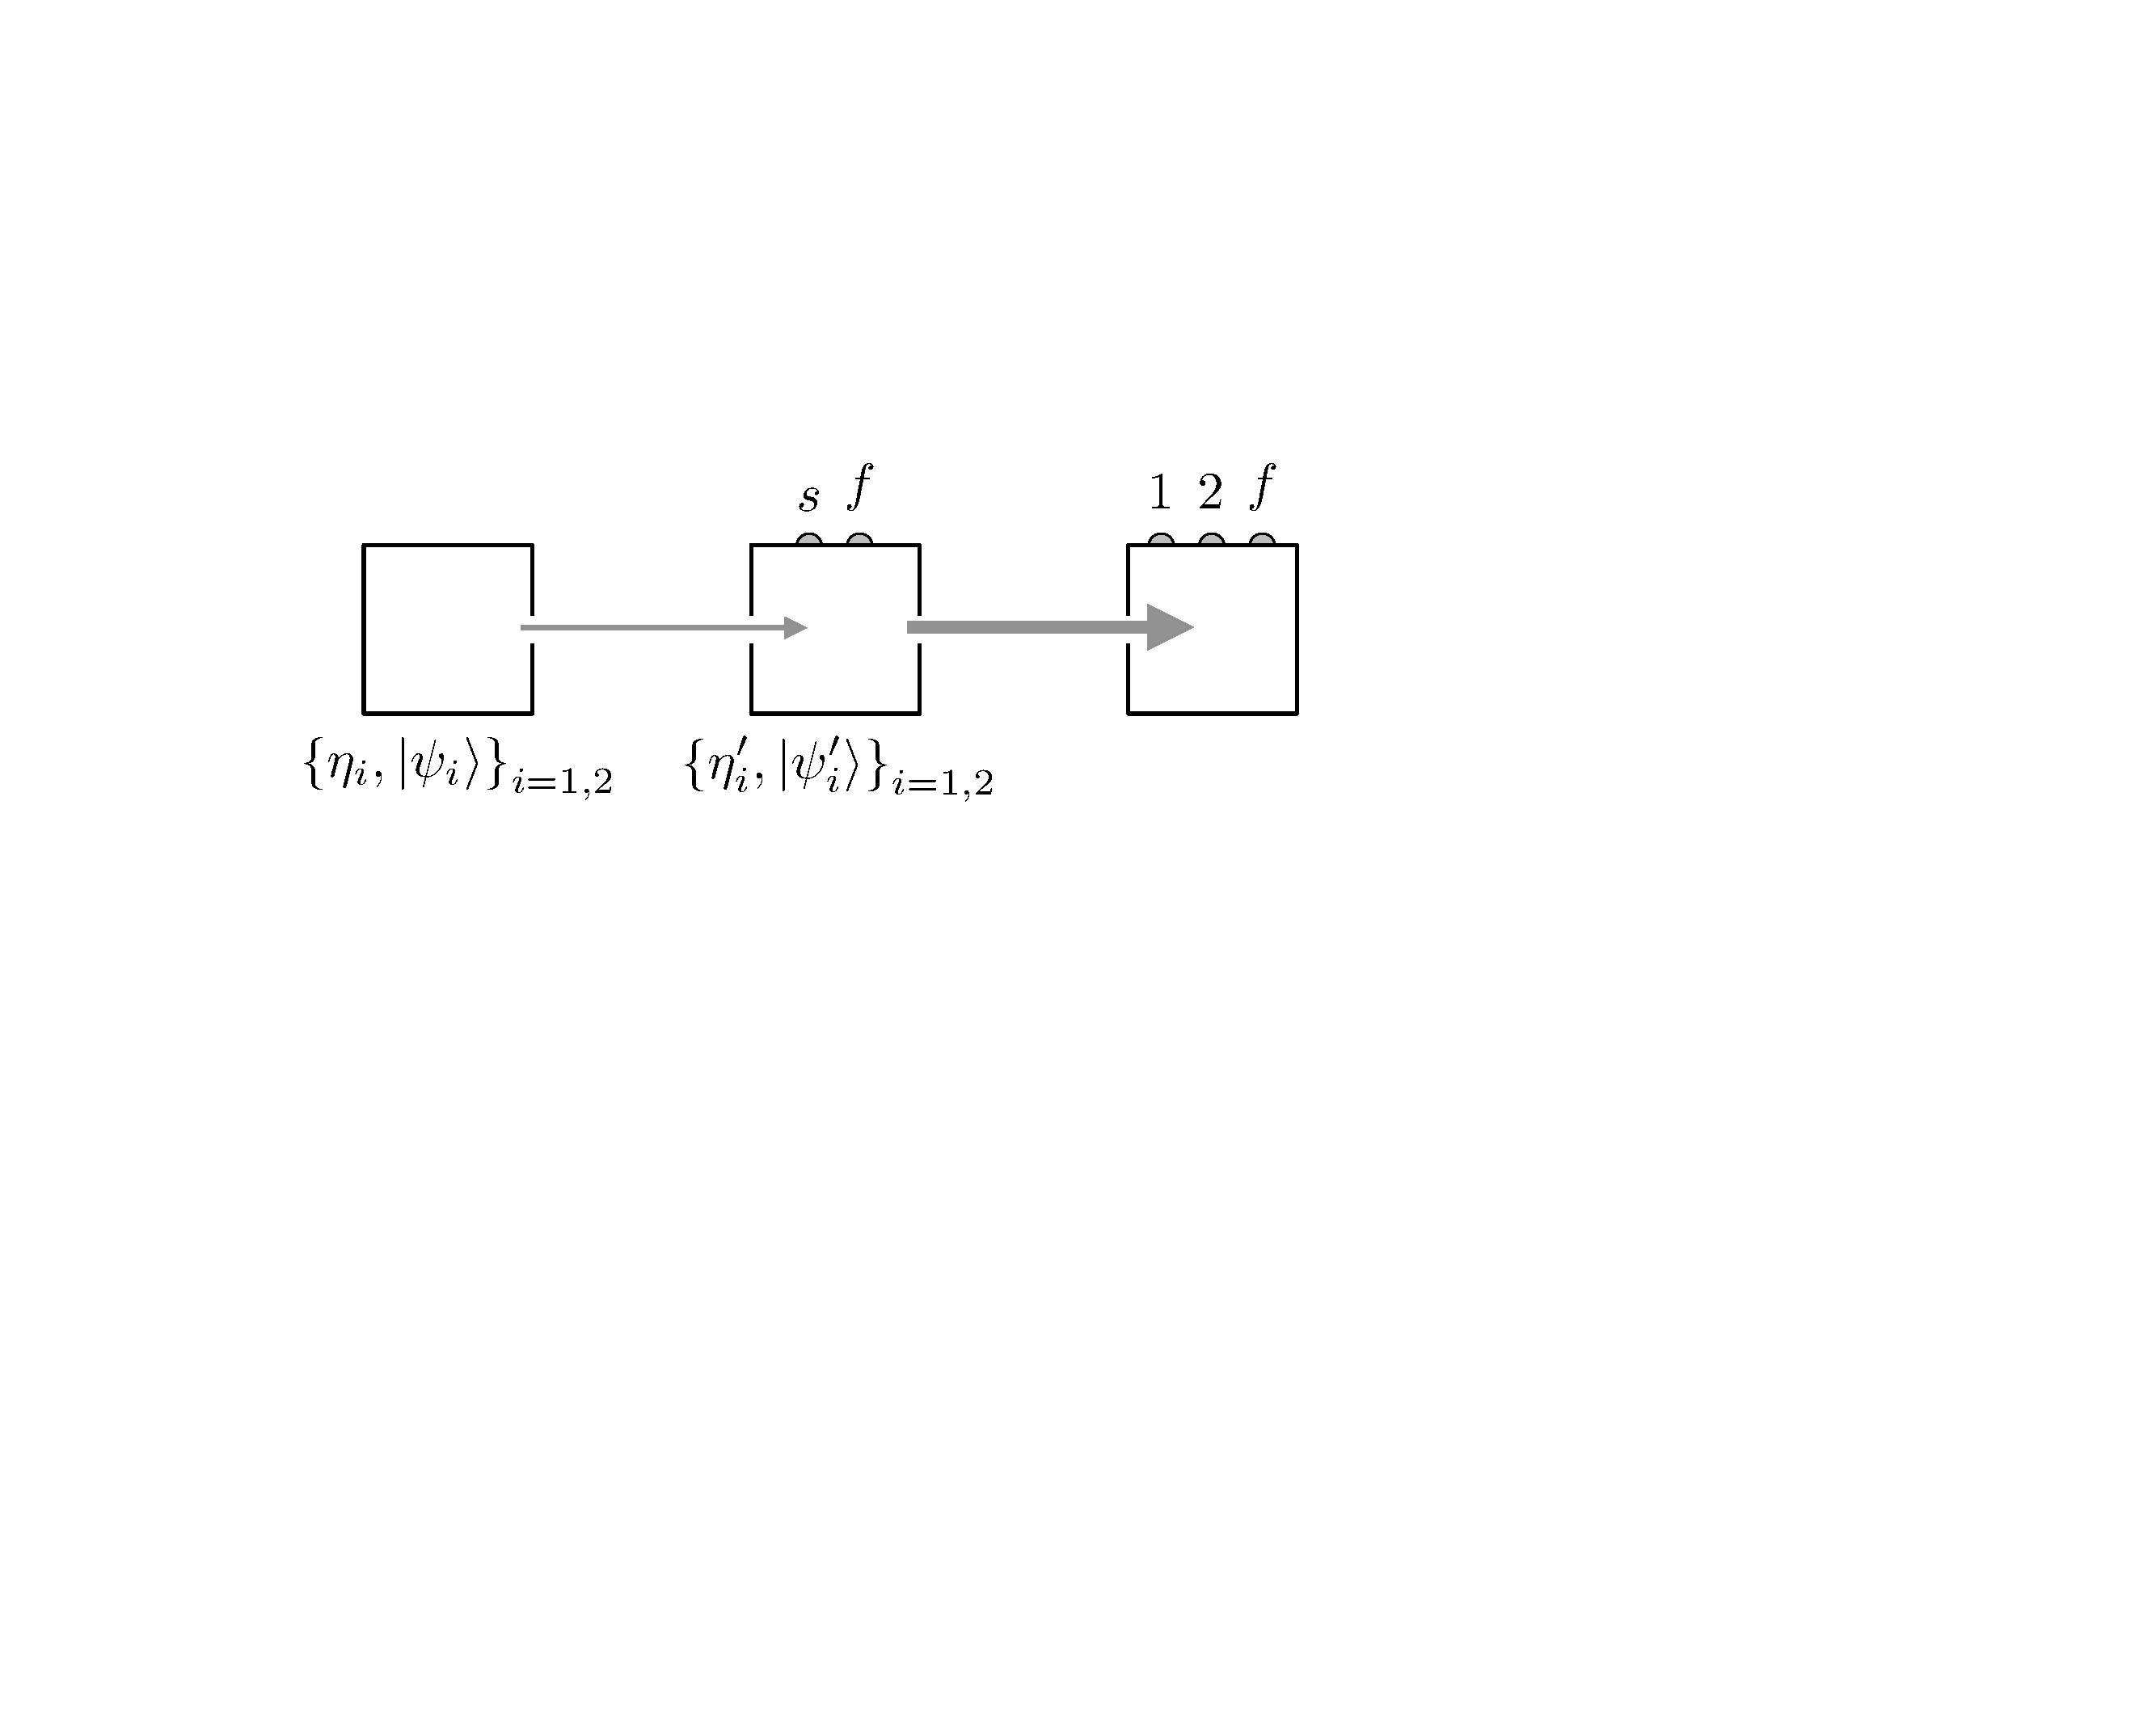
\includegraphics[width=22em]{Vadim_F1.pdf}
$$
The box in the middle has two classical outputs labeled $s$ and $f$ (success and failure). If $f$ is triggered, the two-step discrimination process is aborted and ``failure" is reported. Upon getting $s$, two possible states are produced, $|\psi_i\rangle\to|\psi'_i\rangle$ with {\em conditioned} probability~$\eta'_i$. Let $p_i$ be the success probability if the state $|\psi_i\rangle$ is fed into the central box, then 
$$
\eta'_i={\eta_i p_i\over\eta_1 p_1+\eta_2 p_2}
$$
The information leakage can be quantified as
$$
L=H_2(\eta|s)-H_2(\eta'|s)
$$
where $\eta$ and $\eta'$ are the probability distributions $\{\eta_1,\eta_2\}$ and $\{\eta'_1,\eta'_2\}$ respectively and $H_2$ is the binary Shannon entropy
$$
H_2(\eta|s)=h_2(\eta_1)=-\eta_1\log\eta_1-(1-\eta_1)\log(1-\eta_1)
$$
We note that $x'<x<1/2$ iff $h_2(x')<h_2(x)$. Thus, 
$$
0<\eta_1-\eta'_1
$$
is a condition for information leakage, if we assume $0\le\eta_1\le1/2$ (which we can do without loss of generality).
The condition above is equivalent to
$$
0<\eta_1\left(1-{p_1\over\eta_1 p_1+\eta_2 p_2}\right)={\eta_1\eta_2\over\eta_1 p_1+\eta_2 p_2}(q_1-q_2)
$$
Then
$$
l\equiv\eta_1(q_1-q_2)>0
$$
(as $\eta_2\ge 1/2$) is a quantitative measure (most likely convenient for this kind of problem) of the information leakage.
We note that if the central box is a ``cloning machine", the leakage $l$ is zero iff $\eta_1=0$ or $\eta_1=\eta_2=1/2$, since this is equivalent to $q_1=q_2$.

It would be nice to prove that for a generic box in the middle (not necessarily a cloning machine), the condition $l>0$ necessarily implies that the two step discrimination process is suboptimal. Ideally, we would like to have a proof for {\em any} box, not necessarily a binary one. This may be a lot more complicated, since in this case $H(\eta')$ is not binary.  A proof for binary boxes should be enough for now. Maybe we can argue that for unambiguous discrimination we can always lump together the various Klauss operators in the box in two groups: success and failure...

%
\begin{eqnarray*}
U|\psi_1\rangle|0\rangle&=& \sqrt{p_1}|\Psi_1\rangle|\alpha_1\rangle +\sqrt q_1 |\Phi_1\rangle\\
U|\psi_2\rangle|0\rangle&=& \sqrt{p_2}|\Psi_2\rangle|\alpha_2\rangle +\sqrt q_2 |\Phi_2\rangle
\end{eqnarray*}
%
The ``label" space $\mathscr L$ contains 2 orthogonal subspaces $\mathscr S$ and $\mathscr F$ (success and failure respectively). The states $|\alpha_1\rangle$ and $|\alpha_2\rangle$ belong to the success subspace~$\mathscr S$, whereas $\tr_{\!\!\mathscr L}\Phi_1$ and $\tr_{\!\!\mathscr L}\Phi_2$, where  $\tr_{\!\!\mathscr L}$ is the partial trace over everything but the label space, is a density matrix on $\mathscr F$. Therefore, a projective measurement on the label space, $M=\{{\mathbb I}\otimes P_{\mathscr S},{\mathbb I}\otimes P_{\mathscr F}\}$, provide us with conclusive evidence of our success or failure in producing $|\Psi_1\rangle$ or $|\Psi_2\rangle$ (depending on the initial state being $|\psi_1\rangle$ or $|\psi_2\rangle$ respectively). Note that we have
$$
(\tr_{\!\!\mathscr L}\Phi_i)|\alpha_j\rangle=0,\quad i,j=1,2
$$
The unitarity condition is
$$
s=\sqrt{p_1 p_2} s' \alpha+\sqrt{q_1 q_2}\phi
$$
where
$$
s'=\langle\Psi_1|\Psi_2\rangle,\quad \alpha=\langle\alpha_1|\alpha_2\rangle,\quad \phi=\langle\Phi_1|\Phi_2\rangle
$$
We can choose $s,s'\ge0$, but different phases for $\alpha$ and $\phi$ lead to different unitarity conditions. Not, however, that we may choose them to be real, since only their real part are relevant to the unitarity conditions and the additional condition
$$
0=\sqrt{p_1p_2}s' \Im\,\alpha+\sqrt{q_1q_2}\Im\,\phi
$$
can always be met. So, we take $ \Im\,\alpha=\Im\,\phi=0$.
We assume $s>s'$, namely, the posterior states are more distinguishable that the original ones. Then
$$
\phi={s-s'\sqrt{p_1p_2}\alpha\over\sqrt{q_1q_2}}\ge {s-s'\sqrt{p_1p_2}|\alpha|\over\sqrt{q_1q_2}}\ge {s-s'\over\sqrt{q_1q_2}}>0
$$
Actually, we have a stronger condition; proceeding as in Sec.~\ref{uni cur}, we have
$$
s=-{\phi-s'\alpha\over2}x+{\phi+s'\alpha\over2}y
$$
Then, taking absolute values
$$
s\le\left|-{\phi-s'\alpha\over2}x\right|+\left|{\phi+s'\alpha\over2}y\right|={\phi+s'\alpha+|\phi-s'\alpha|\over2}\le\max\left\{\phi,s'|\alpha|\right\}
$$
So necessarily $s\le\phi$, since otherwise $s\le \max\{\phi,s'|\alpha|\}<\max\{s,s'|\alpha|\}=s$. Now, we show that optimality requires $\alpha>0$. Consider the two curves (resp., blue and red in the next figure):
$$
s=s'|\alpha| \sqrt{p_1p_2}+\sqrt{q_1q_2}\phi,\qquad s=-s'|\alpha| \sqrt{p_1p_2} +\sqrt{q_1q_2}\phi
$$
and the straight line 
$$
q_1=\xi_1 t,\quad q_2=\xi_2 t,\qquad \xi_1,\xi_2\ge0,\quad \xi_1^2+\xi_2^2=1
$$
For given $\xi_1$, $\xi_2$, the distance from the origin to $(q_1,q_2)$ is~$t$. Substituting in the equations of the two curves we see from the resulting equation that whenever the straight line intersects the curve with negative $\alpha$ it also intersects the other. If $t_+$, $t_-$ give intersecting points for positive and negative $\alpha$ respectively, we have
$$
t_+\!=\!{s\!-\!|\alpha|s'\!\sqrt{1\!-\!\xi_1 t_+}\sqrt{1\!-\!\xi_2 t_+}\over\phi\sqrt{\xi_1\xi_2}}\le\!
{s\over\phi\sqrt{\xi_1\xi_2}}
\le\!
{s\!+\!|\alpha|s'\!\sqrt{1\!-\!\xi_1 t_-}\sqrt{1\!-\!\xi_2 t_-}\over\phi\sqrt{\xi_1\xi_2}}\!=\!t_-
$$
Hence, the straight line $Q=\eta_1 q_1+\eta_2 q_2$ will intersect the curve with $\alpha=-|\alpha|$ for larger values of $Q$ than it will intersect that with $\alpha=|\alpha|$.
$$
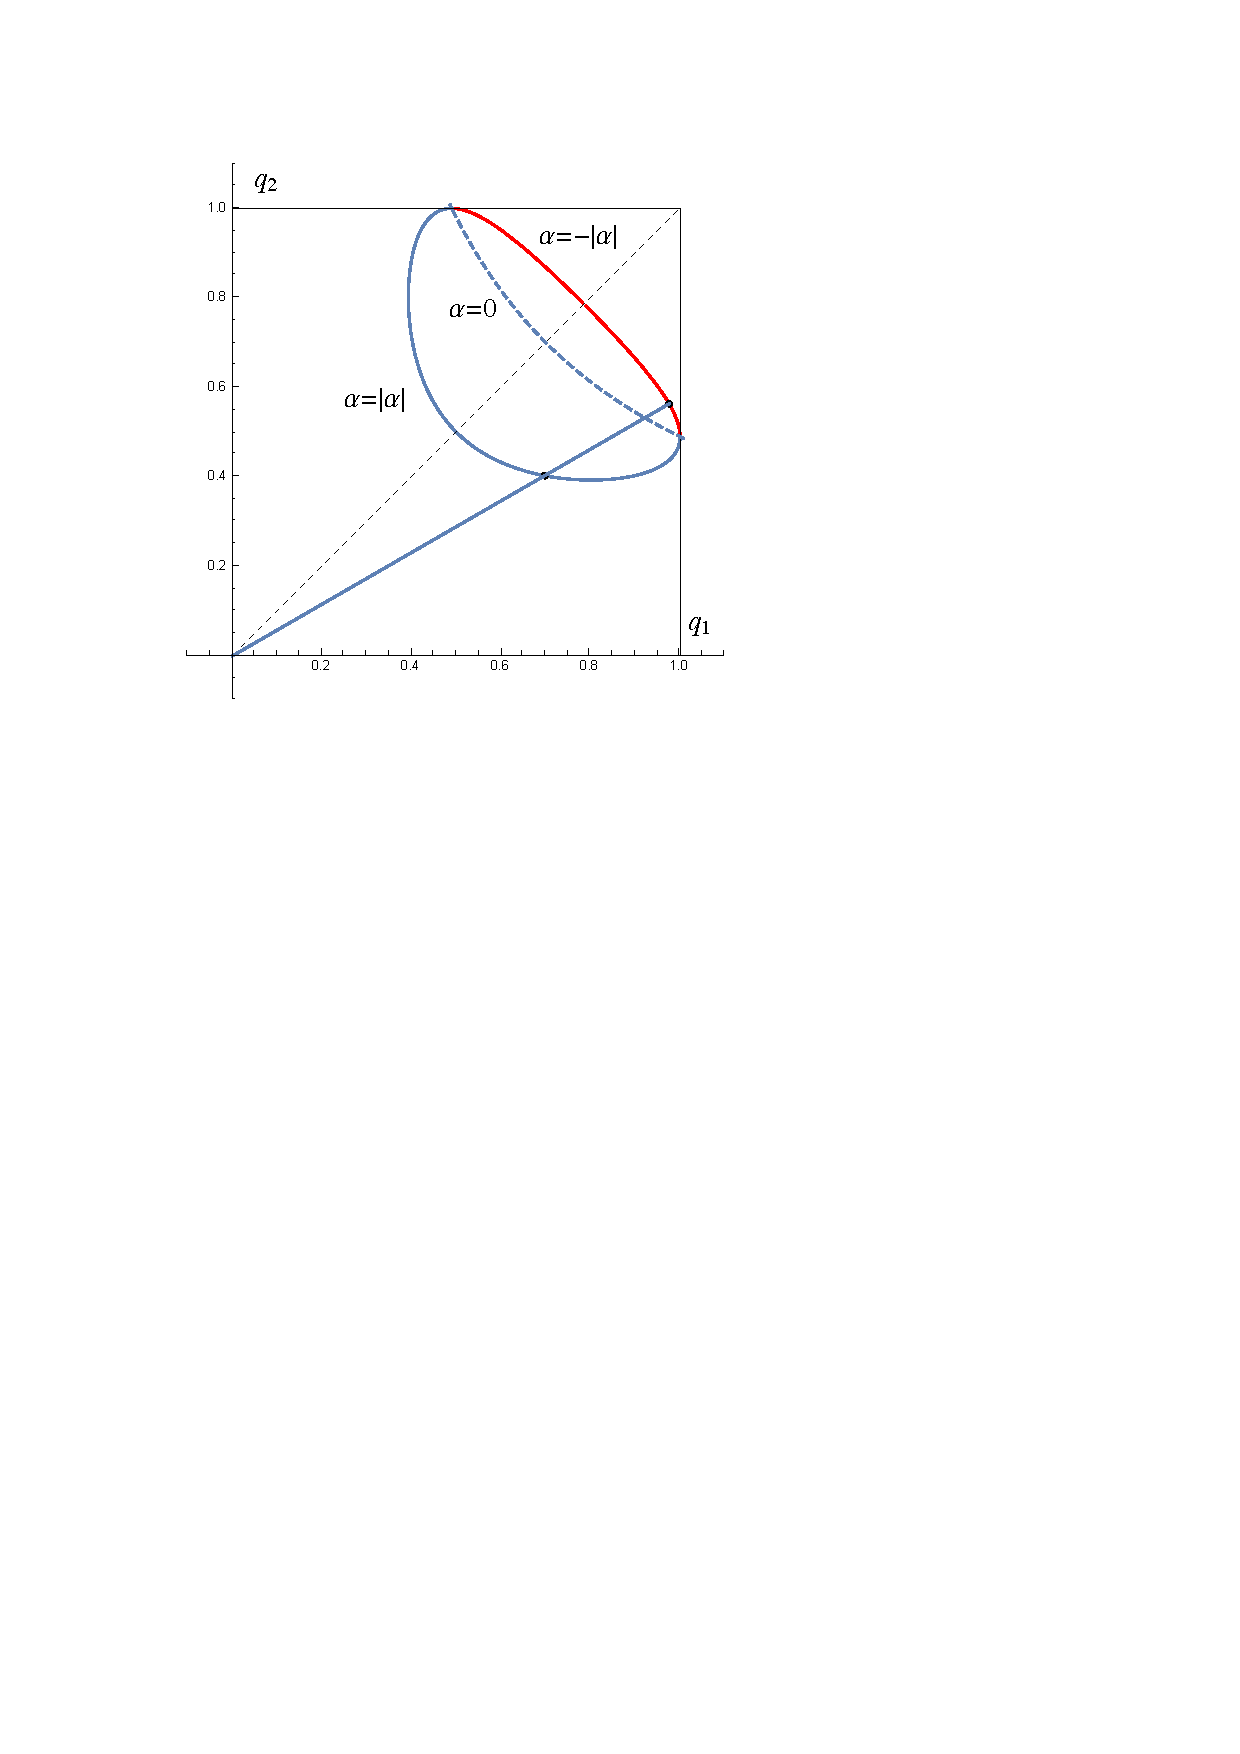
\includegraphics[width=22em]{Andi4_F3.pdf}
$$
The limiting curve as $\alpha\to0$ is given by $t_0=s/(\phi\sqrt{\xi_1\xi_2})$. Therefore, it is the Unambiguous discrimination hyperbola 
$$
q_1 q_2=(\xi_1t_0)(\xi_2 t_0)={s^2\over\phi^2}
$$
It is also clear from this picture that $t_+$ ($t_-$) is a decreasing (increasing) function of $|\alpha|$, Hence, the minimum value of $Q$ is given by $\alpha=1$, which implies that~$|\alpha_1\rangle=|\alpha_2\rangle$. Similarly, $\phi=1$, and hence $|\Phi_1\rangle=|\Phi_2\rangle$ is the optimal choice.

A convenient symmetric parametrization is
$$
x={1-(\phi+\alpha s')t\over \alpha s'/s};\qquad y={1-(\phi-\alpha s')t\over \alpha s'/s}
$$
The range of $t$ is given by the intersection of
$$
{1-\alpha s'/s\over\phi+\alpha s'}\le t\le{1+\alpha s'/s\over\phi+\alpha s'};\qquad
{1-\alpha s'/s\over\phi-\alpha s'}\le t\le{1\over\phi-\alpha s'};\qquad 
t\le{1\over\phi}
$$
We have
$$
{1-\alpha s'/s\over\phi-\alpha s'}\le t\le {1\over\phi}
$$


\end{document}